%% LyX 2.2.3 created this file.  For more info, see http://www.lyx.org/.
%% Do not edit unless you really know what you are doing.
\documentclass[english]{article}
\usepackage{mathptmx}
\usepackage{helvet}
\usepackage{courier}
\usepackage[T1]{fontenc}
\usepackage[latin9]{inputenc}
\usepackage{geometry}
\geometry{verbose,tmargin=1in,bmargin=1in,lmargin=1in,rmargin=1in,headheight=0in,headsep=0in}
\pagestyle{empty}
\usepackage{color}
\usepackage{babel}
\usepackage{listings}
\usepackage{graphicx}
\usepackage[unicode=true]
 {hyperref}

\makeatletter

%%%%%%%%%%%%%%%%%%%%%%%%%%%%%% LyX specific LaTeX commands.
%% Because html converters don't know tabularnewline
\providecommand{\tabularnewline}{\\}

%%%%%%%%%%%%%%%%%%%%%%%%%%%%%% Textclass specific LaTeX commands.
\newenvironment{lyxcode}
{\par\begin{list}{}{
\setlength{\rightmargin}{\leftmargin}
\setlength{\listparindent}{0pt}% needed for AMS classes
\raggedright
\setlength{\itemsep}{0pt}
\setlength{\parsep}{0pt}
\normalfont\ttfamily}%
 \item[]}
{\end{list}}

%%%%%%%%%%%%%%%%%%%%%%%%%%%%%% User specified LaTeX commands.
\date{}

\makeatother

\begin{document}
\begin{center}
\textbf{\large{}CSCE 221 Assignment 3 Cover Page}\\
\bigskip{}
\par\end{center}

First Name~~Hunter~~~~~~~~~~Last
Name ~~~Cleary~~~~~~~~UIN~~625001547~~\bigskip{}

User Name ~~~hncleary~~~~E-mail
address~~~~hncleary@tamu.edu~~~\medskip{}

Please list all sources in the table below including web pages which
you used to solve or implement the current homework. If you fail to
cite sources you can get a lower number of points or even zero, read
more on Aggie Honor System Office website: \texttt{\href{http://aggiehonor.tamu.edu/}{http://aggiehonor.tamu.edu/}}\medskip{}
\medskip{}
\noindent \begin{flushleft}
\begin{tabular}{|c|c|c|c|c|}
\hline 
Type of sources  & ~~~~~~~~~~~~~~~~~~~~~~~ & ~~~~~~~~~~~~~~~~~~~~~~~~ & ~~~~~~~~~~~~~~~~~~~~~~~ & ~~~~~~~~~~~~~~~~~~~~~~~\tabularnewline
 &  &  &  & \tabularnewline
\hline 
People &  &  &  & \tabularnewline
 &  &  &  & \tabularnewline
\hline 
Web pages (provide URL)  & Listed Below  &  &  & \tabularnewline
 &  &  &  & \tabularnewline
\hline 
Printed material & Data Structures and Algorithms &  &  & \tabularnewline
 & (Textbook) &  &  & \tabularnewline
\hline 
Other Sources  &  &  &  & \tabularnewline
 &  &  &  & \tabularnewline
\hline 
\end{tabular}
\par\end{flushleft}\ \\ 
\ \\
\textbf{Websites}\ \\ 
https://en.wikipedia.org/wiki/Doubly\_linked\_list\ \\
https://www.geeksforgeeks.org/doubly-linked-list/\ \\
https://stackoverflow.com/questions/32938119/doubly-linked-list-insert-before-function-c\ \\
\ \\
\medskip{}
\medskip{}

\noindent I certify that I have listed all the sources that I used
to develop the solutions/codes to the submitted work.

\noindent \emph{On my honor as an Aggie, I have neither given nor
received any unauthorized help on this academic work}.

\bigskip{}
\bigskip{}

\begin{tabular}{cccccc}
Your Name  & ~~~Hunter Cleary~~ &  & ~~~~~~~~~~~~~~~~~~~~~ & Date  & ~~~3-8-18~~\tabularnewline
\end{tabular}

\newpage
%\title{The Programming Assignment Report Instructions\\
%CSCE 221}
\begin{enumerate}
\item The description of an assignment problem.\ \\ 
\ \\
The assignment required that a doubly linked list classes be created and implemented in C++. The first class was created for integer data types. A second, templated, class was created for data of arbitrary type. A MinQueue data structure was also created that supports queue operations and a min() function.
\ \\
\item The description of data structures and algorithms used to solve the
problem.
\begin{enumerate}
\item Provide definitions of data structures by using Abstract Data Types
(ADTs)\ \\ \ \\
A doubly linked list is a set of nodes that each hold two pointers. The pointers of each node point to the previous node and the next node. Typically there also exists a search node which is able to traverse the list. The pointers between data nodes allow the search node to move in both directions. Doubly linked lists allow for optimized insertion, deletion, and access at any node.


\ \\
\item Write about the ADTs implementation in C++.\ \\ \ \\
The DoublyLinkedList class in C++ contains a set of functions that work with the DListNode Structure. DListNode contains the stored data and the pointers to the previous and proceeding node. The DoublyLinkedList Class contains functions for various forms of output, insertion, and removal. It also contains a copy constructor for moving nodes into a new list and destrcutor for deleting the items. 


\ \\
\item Describe algorithms used to solve the problem.\ \\
\ \\
Linear search was used several times to find desired nodes in order to insert / delete at a specific point in the list. A function was created to find minimum values, which iterates through the list and compares at each node. 

\ \\ 
\item Analyze the algorithms according to assignment requirements. \ \\
 \textbf{Doubly Linked List}\ \\   
 insertFirst - O(1) - Inserts a node at the beginning of the list. Creates a new node and then reassigns the pointer.\ \\
 insertLast - O(1) - Functions the same way as insertFirst, but at the end of the list.\ \\
 removeFirst - O(1) - Deletes the first node and reassigns the pointer of the next node.\ \\
 removeLast - O(1) - Deletes the last node and reassigns the pointer of the previous node.\ \\
 first(),last() - O(1) - Checks the value of the first / last node.\ \\ 
 isEmpty - O(1) - Makes a comparison to see if the list is NULL.\ \\
 Copy Constructor - O(n) - The function copies every item and places it into another list.\ \\
 Output Operator - O(n) - Prints out each node in the list.\ \\
 ListLength - O(n) - Iterates through the list and counts the number of items present.\ \\
 insertAfter, insertBefore - O(n) - Searches through the list for a specific node and then places it before / after. Reassigns corresponding pointers.\ \\
 removeBefore, removeAfter - O(n) - Searches through the list for a specific node and then deletes the node before / after it. Reassigns pointers to compensate for missing node.\ \\
\textbf{MinQueue}\ \\
enqueue - O(1) - Inserts node at the start of the queue.\ \\
dequeue - O(1) - Removes node from the end of the queue.\ \\
isEmpty - O(1) - Makes a comparison to see if the list is NULL.\ \\
min - O$(n^2)$ - Looks at each value of the list, makes copmarisons and the outputs the smallest value in the list.\ \\


\ \\
\end{enumerate}
\item A C++ organization and implementation of the problem solution 
\begin{enumerate}
\item Provide a list and description of classes or interfaces used by a
program such as classes used to implement the data structures or exceptions.
\ \\ \ \\
DoublyLinkedList - class for doubly linked list containing integer values\ \\
TemplateLinkedList - class for doubly linked list containing generic data types\ \\
MinQueue - wrapper for doubly linked list that enables queue functions \ \\
\ \\
\item Include in the report the class declarations from a header file (.h)
and their implementation from a source file (.cpp).\ \\
\begin{lstlisting}
#include <cstdlib>
#include <iostream>
using namespace std;
class DoublyLinkedList; // class declaration

// list node
struct DListNode {
  int obj;
  DListNode *prev, *next;
  DListNode(int e=0, DListNode *p = NULL, DListNode *n = NULL)
    : obj(e), prev(p), next(n) {}
  int getElem() const { return obj; }
  DListNode * getNext() const { return next; }
  DListNode * getPrev() const { return prev; }
};

// doubly linked list
class DoublyLinkedList {
private:
  DListNode header, trailer;
public:
  DoublyLinkedList() : header(0), trailer(0) // constructor
  { header.next = &trailer; trailer.prev = &header; }
  DoublyLinkedList(const DoublyLinkedList& dll); // copy constructor
  ~DoublyLinkedList(); // destructor
  DoublyLinkedList& operator=(const DoublyLinkedList& dll); // assignment operator
  // return the pointer to the first node
  DListNode *getFirst() const { return header.next; } 
  // return the pointer to the trailer
  const DListNode *getAfterLast() const { return &trailer; }
  // return if the list is empty
  bool isEmpty() const { return header.next == &trailer; }
  int first() const; // return the first object
  int last() const; // return the last object
  void insertFirst(int newobj); // insert to the first of the list
  int removeFirst(); // remove the first node
  void insertLast(int newobj); // insert to the last of the list
  int removeLast(); // remove the last node
  void insertAfter(DListNode &p, int newobj); // insert after desired node
  void insertBefore(DListNode &p, int newobj); // insert before selected node
  int removeAfter(DListNode &p); // removes node after selected
  int removeBefore(DListNode &p); //removes node before selected
};

// output operator
ostream& operator<<(ostream& out, const DoublyLinkedList& dll);
// return the list length
int DoublyLinkedListLength(DoublyLinkedList& dll);
\end{lstlisting}

\ \\
\item Provide features of the C++ programming paradigms like Inheritance
or Polymorphism in case of object oriented programming, or Templates
in the case of generic programming used in your implementation.
\ \\ \ \\
TemplateDoublyLinkedList is templated version of the DoublyLinkedList class. The new class allows for any input of generic type T. The original class was altered using template<class T> to allow for the generic input.
\ \\
\end{enumerate}
\item A user guide description how to navigate your program with the instructions
how to: 
\begin{enumerate}
\item compile the program: specify the directory and file names, etc.\ \\
\ \\
Each directory (DoublyLinkedList, TemplateDoublyLinkedList, and MinQueue) has a make file. 
\ \\
\item run the program: specify the name of an executable file.\ \\
\ \\
Once compiled, the programs should run with:\
./Main, 
 ./TemplatedMain, and
 ./MinQueue,
respectively.
\ \\
\end{enumerate}
\item Specifications and description of input and output formats and files \ \\
\ \\
All files run solely in the command line once compiled.
\ \\
\item Provide types of exceptions and their purpose in your program.\ \\

\begin{enumerate}
\item logical exceptions (such as deletion of an item from an empty container,
etc.)
\ \\ \ \\
The program avoids using nodes that are NULL. There are several safeguards implemented so that memory is properly handled.
\ \\
%\item runtime exception (such as division by $0$, etc.)\vfill{}
\end{enumerate}

\newpage
\item Test your program for correctness using valid, invalid, and random
inputs (e.g., insertion of an item at the beginning, at the end, or
at a random place into a sorted vector). Include evidence of your
testing, such as an output file or screen shots with an input and
the corresponding output.\ \\ \ \\
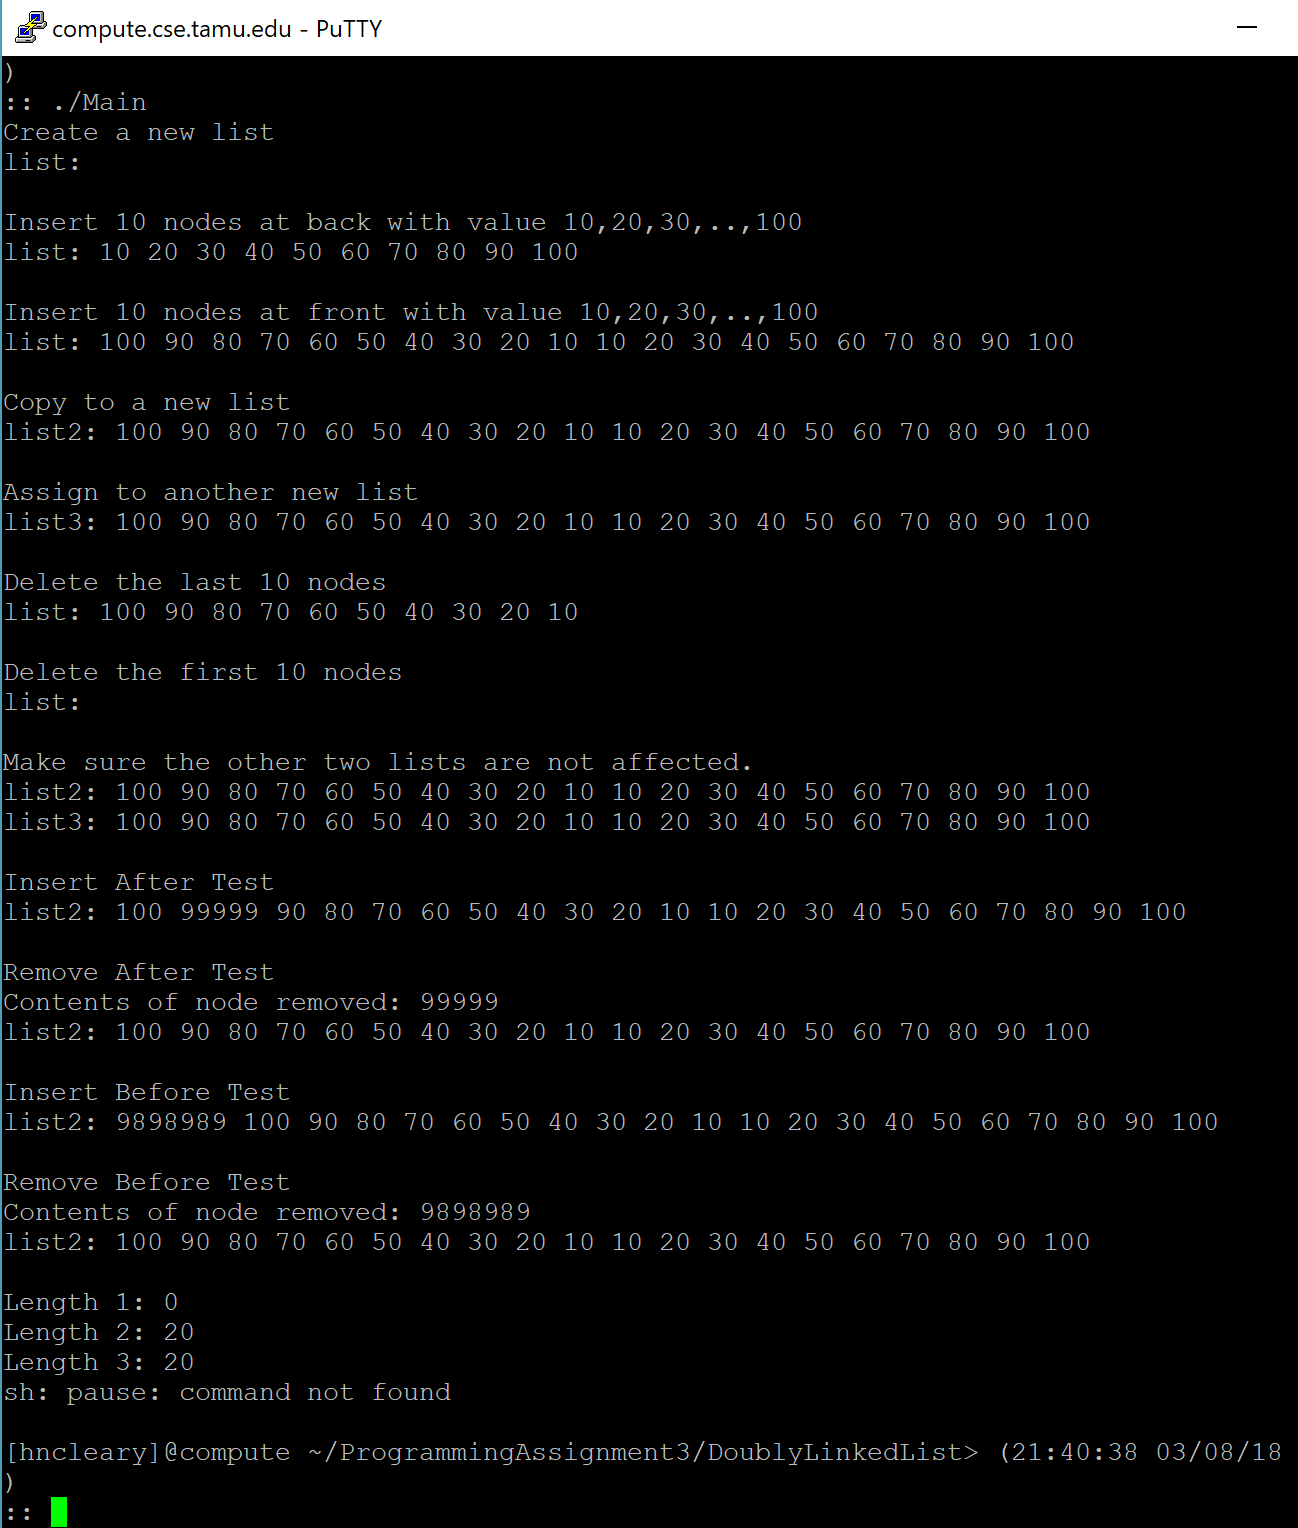
\includegraphics[width=\textwidth,height=\textheight,keepaspectratio]{Main.png}\ \\
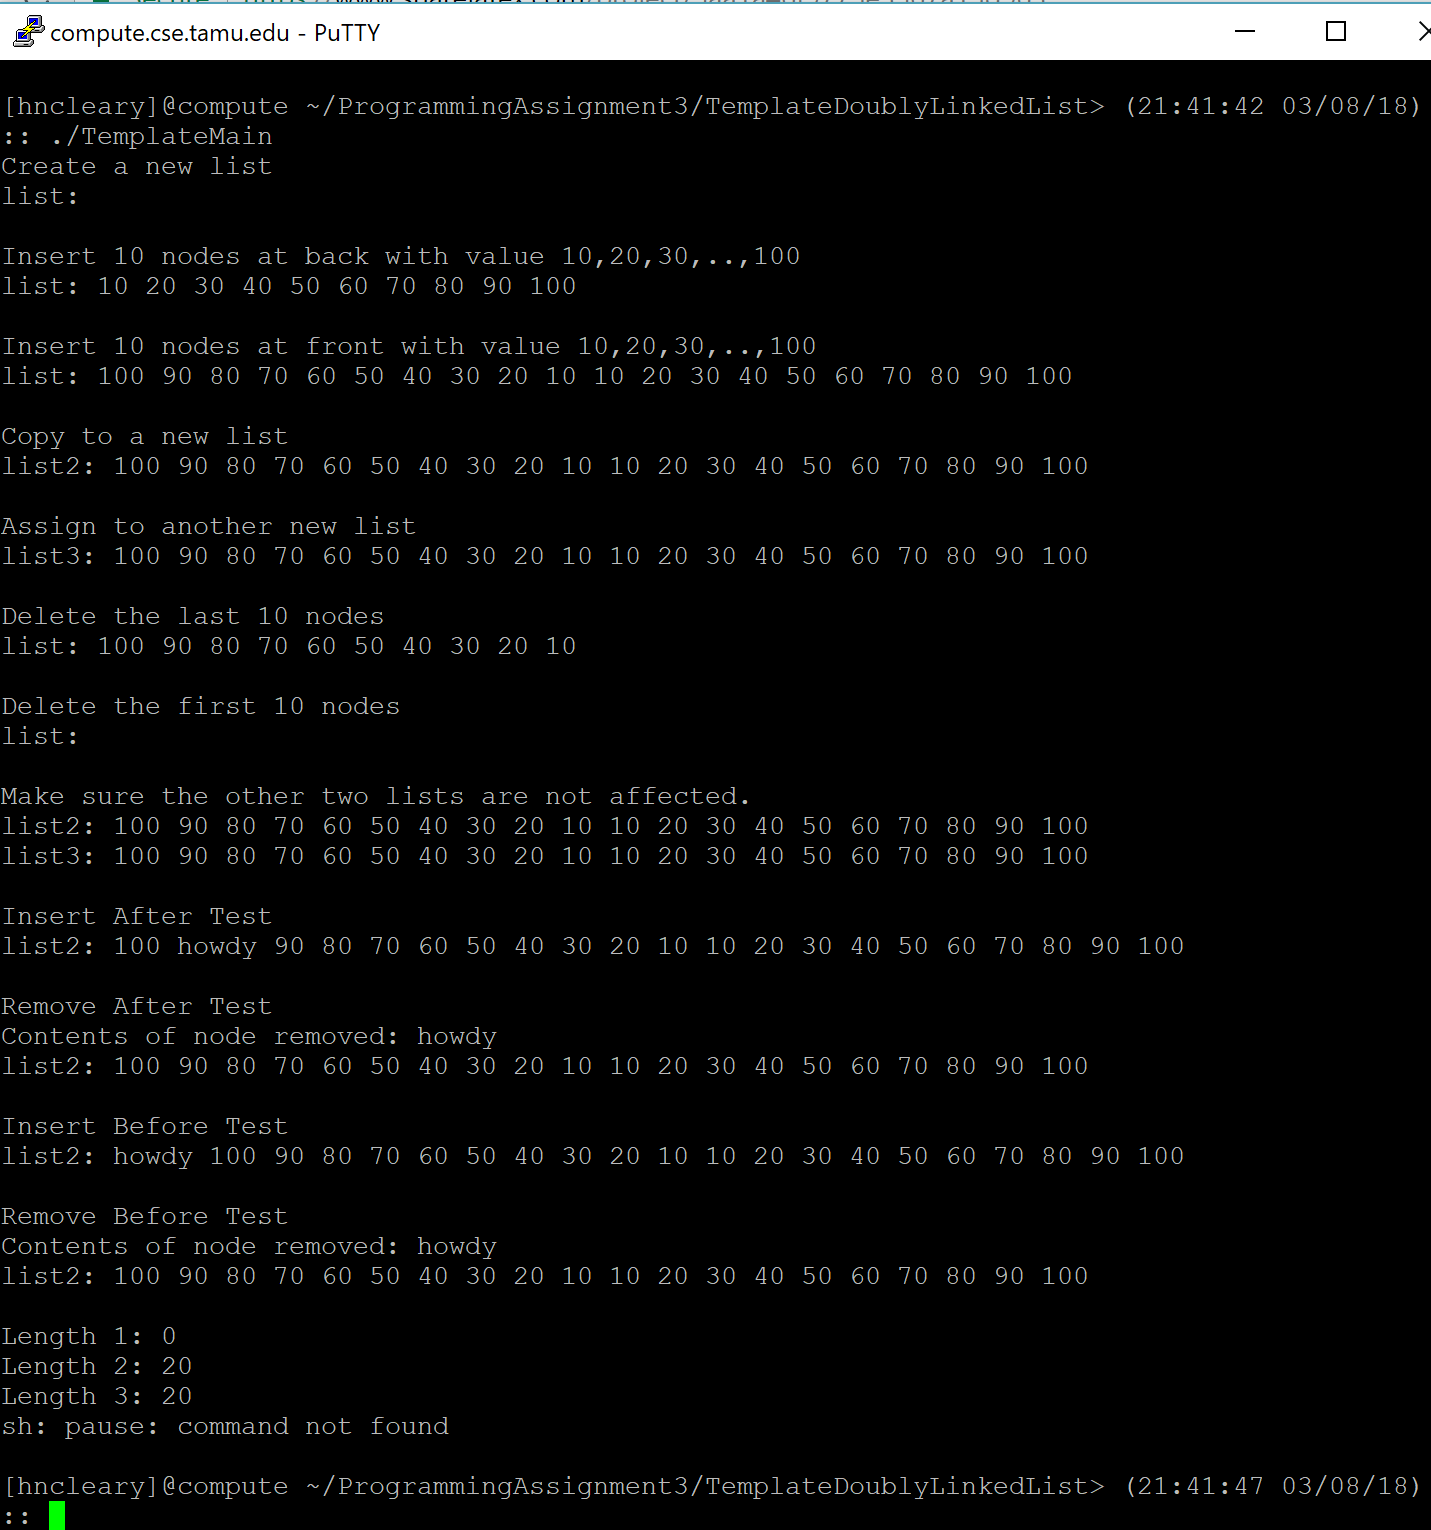
\includegraphics[width=\textwidth,height=\textheight,keepaspectratio]{TemplateMain.png}\ \\
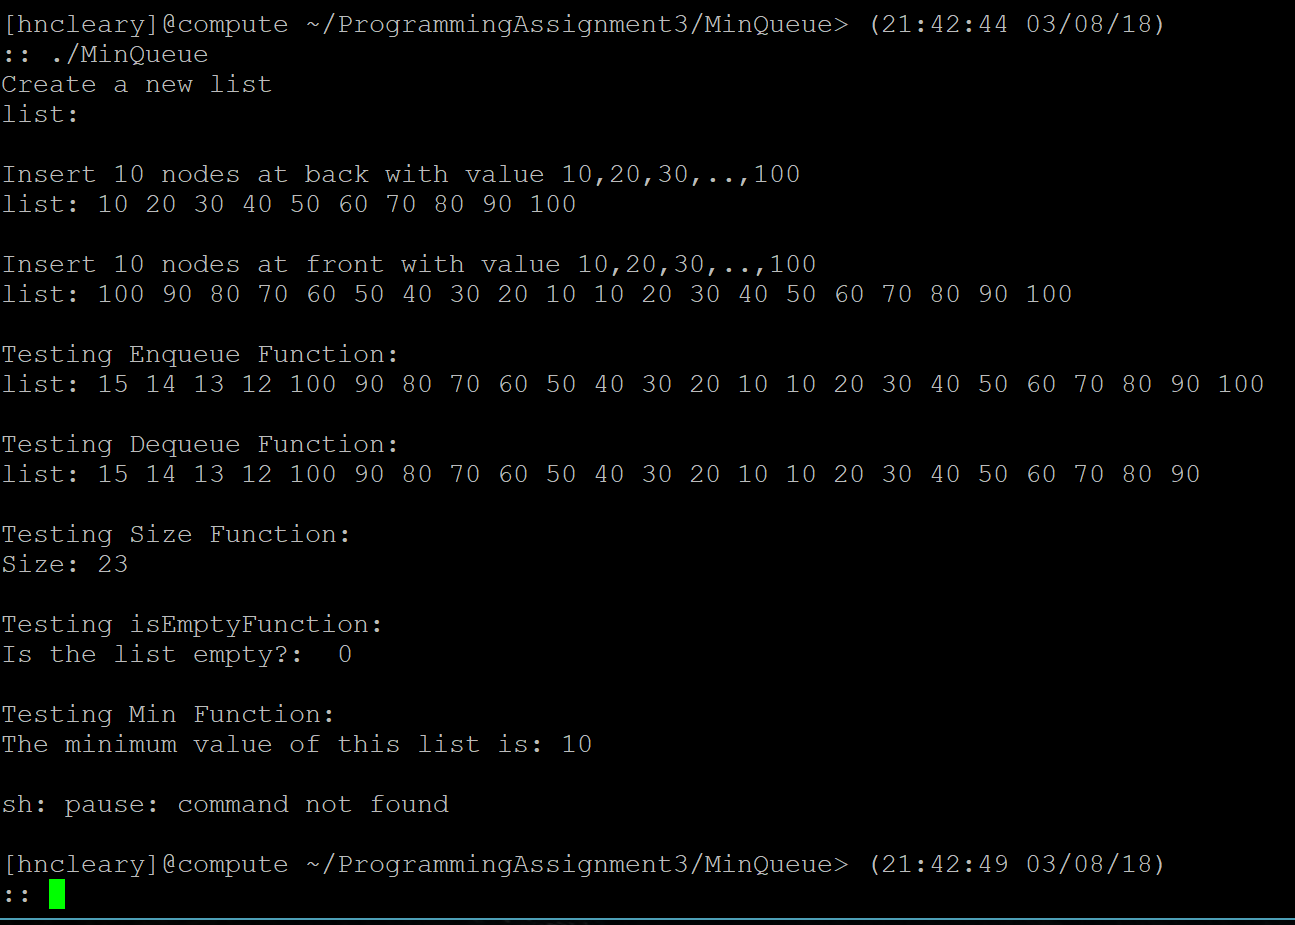
\includegraphics[width=\textwidth,height=\textheight,keepaspectratio]{MinQueue.png}\ \\



\end{enumerate}

\end{document}
